
% ***************************************************
% Example of an internal chapter
% ***************************************************
%This is an internal chapter of the thesis.
%If you have a long title, you can supply an abbreviated version to print in the Table of Contents using the optional argument to the \chapter command.
\chapter[Design overview]{Design overview}
\label{chap:methodology}	%CREATE YOUR OWN LABEL.
\pagestyle{headings}

This chapter details the design decisions and steps taken to complete the project. The project itself can be broken down into three main areas: hardware, firmware and software. 


\section{Hardware}
\subsection{FPGA}
Digilent, parented by National Instruments, make a wide range of Xilinx based FPGA development boards and test equipment. In this project, the Digilent Nexys A7-100T FPGA development board (figure \ref{fig:fpga_dev_board}) was used due to it's availability and features including: a Xilinx Artix 7 100T FPGA (part number XC7A100T-1CSG324C), LAN8720A 100MBit/s RMII PHY, micro SD card slot and PMOD (auxiliary outputs) among other IO. 

Xilinx has multiple FPGAs in their 7-series lineup with different target audiences. The Artix-7 family is optimised for low power designs with high logic throughput. The XC7A100T has 101,440 logic cells, 4,860Kbits of Block RAM (BRAM) and 240 DSP blocks \cite{Xilinx7SeriesDatasheet}. There is a variant of the Nexys A7 FPGA board that consists of a XC7A50T FPGA (fewer resources), but ultimately the XC7A100T variant was used due to its larger amount of resources.  

Importantly, there are four ways this FPGA can be configured (essentially \textit{'programmed'}), at each power on cycle using JTAG, nonvolatile SPI flash, microSD card or using a USB stick through the HID interface. These modes are switchable using jumpers, JP1 and JP2, on the board. The JTAG interface is ideal for testing and as such it was used throughout development process, while storing these configurations on a microSD card was used once the design was solidified. 

\begin{figure}[h!]
    \centering
    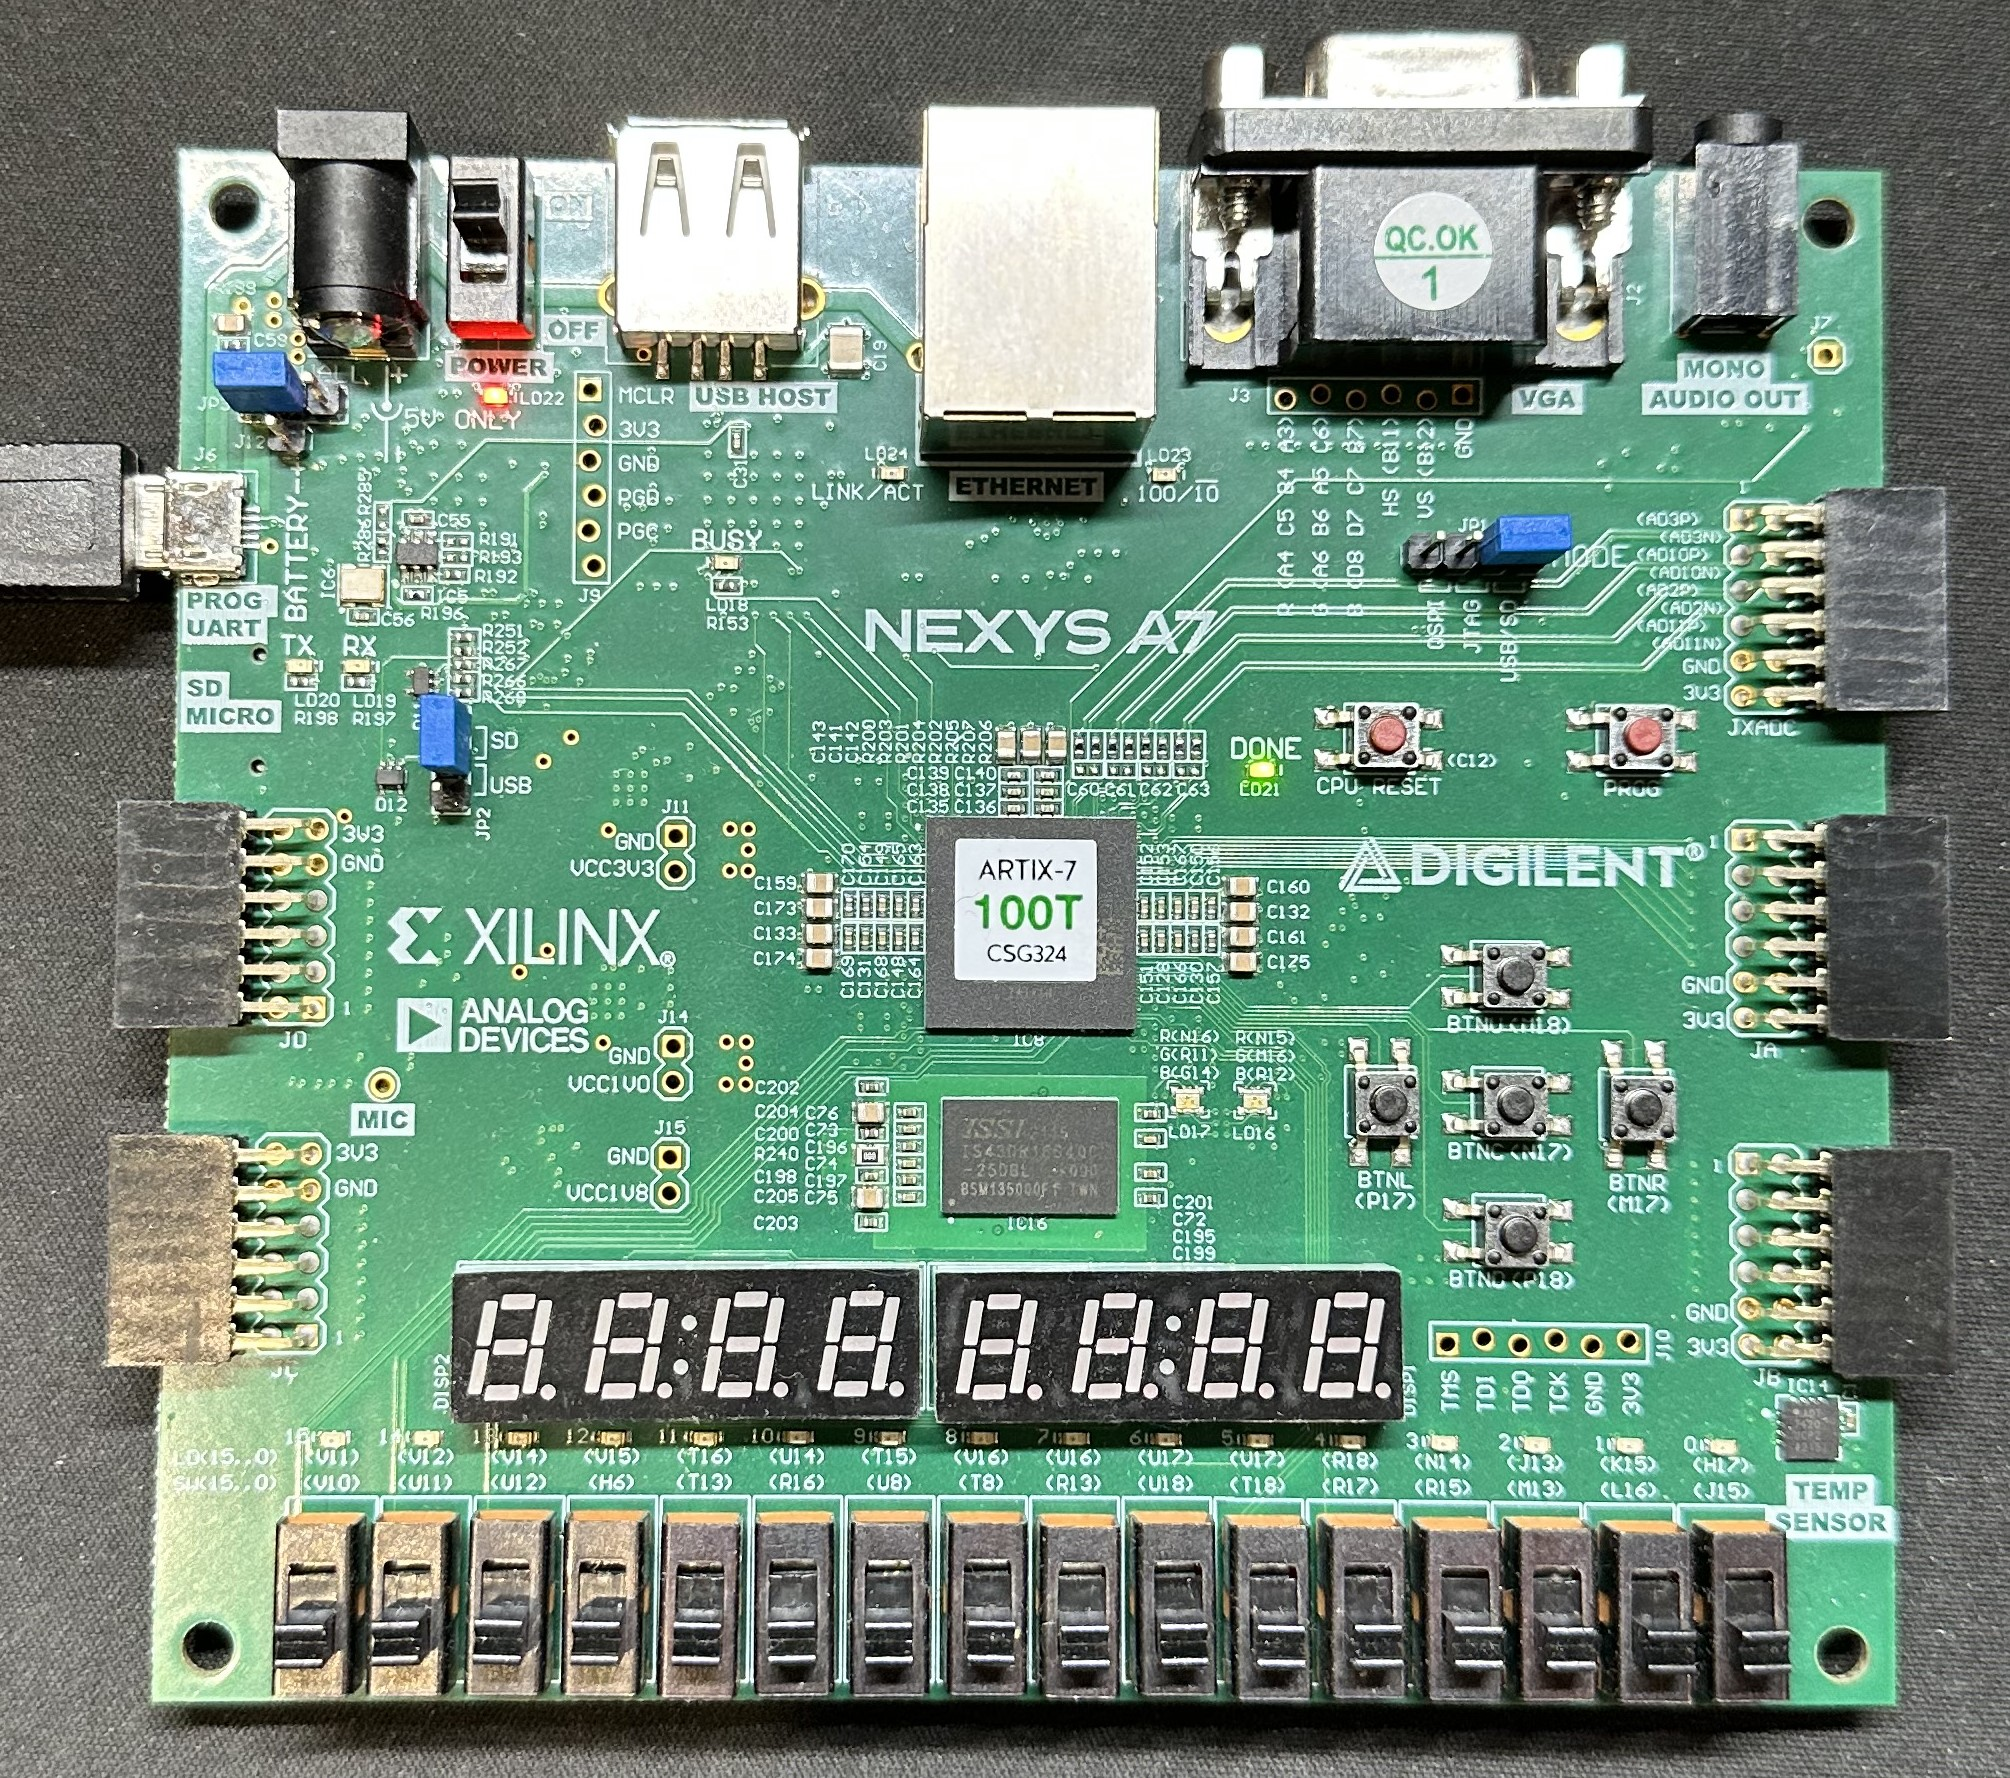
\includegraphics[width=0.65\textwidth]{Images/nexysa7_board.jpg}
    \caption[Digilent Nexys A7 FPGA development board]{Digilent Nexys A7 FPGA development board.}
    \label{fig:fpga_dev_board}
\end{figure}

\newpage






\subsection{MicroSD card}

After the FPGA has been configured using the microSD card, the onboard microcontroller on the Nexys A7 board power cycles the microSD card and relinquishes control of the bus. On power up of the RISC-V softcore processor, it has full control of the card. 

The selected MicroSD card for use in this project is the Patriot LX Series 32GB card, seen in figure \ref{fig:microsd_card}. SD cards, like the patriot card have 2 modes of operation: native SDIO mode and SPI mode. While the native SDIO mode allows for higher speeds, it adds complexity to the design. As the files stored on the SD card are minimal ($< 100KB$), to keep things simple, the microSD card was connected in SPI mode.

\begin{figure}[h]
    \centering
    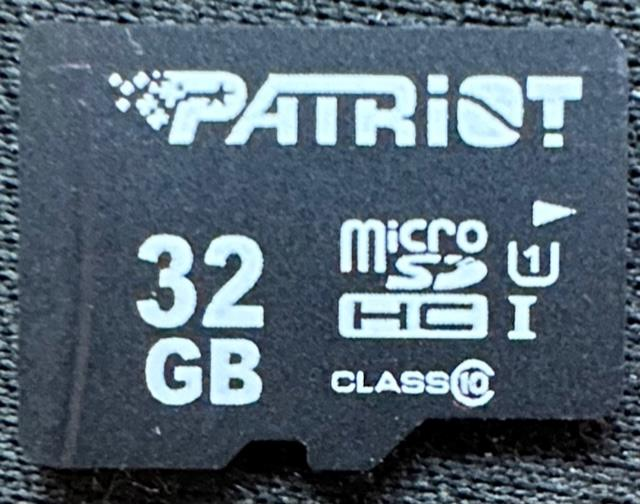
\includegraphics[width=0.2\textwidth]{Images/microsdcard.jpeg}
    \caption[MicroSD card used in project]{MicroSD card used in project.}
    \label{fig:microsd_card}
\end{figure}


\noindent The files that were stored on the microSD card include the bitstream file for the FPGA itself and web assets for the webserver. While the bitstream file needed to be at the root directory of the filesystem, the web assets were stored in their own folder structure to help segregate the files.  








 
\subsection{System on Chip}

A benefit to using an FPGA is that full control is given to the overall system design. At the heart of the SoC, a NEORV32 softcore processor\footnote[1]{See: https://github.com/stnolting/neorv32} controls the hardware and runs the higher layers of the network and webserver tasks.

The NEORV32 processor is RISC-V compatible and designed by GitHub user \textit{stnolting} and is highly configurable. In this design, seen in figure \ref{fig:soc_architecture}, the Wishbone, SPI, UART and external interrupts interfaces were enabled and configured. In addition to these, the M extension (Multiplier) was configured to use the DSP blocks to reduce the number of LUTs needed to handle multiplication in the core. 

The Wishbone B4 classic bus is an open source interface that allows for multiple bits of hardware to connect and communicate together. In this project, the bus is 32bits wide and clocked at 80MHz, giving a bandwidth of $32 \times 80 \times 10^6 = 2.56\times 10^9bit/s=2.56Gbit/s$. Due to its relatively high bandwidth, it was used to connect the MAC with the NEORV32 as packets of 1500 bytes would need to be transferred quickly to not bottleneck the 100Mbit Ethernet interface. In addition to this, the MAC had an interrupt line to the NEORV32 processor to notify it when a packet has been received and ready for processing in the higher layers. This connects into the XIRQ lines which creates a fast interrupt request by firing a mcause trap event (RISC-V terminology).

Serial peripheral Interface (SPI) was used to connect to both the MicroSD card and Packet classifier. These are comparatively low speed and low priority peripherals and so do not require a high speed interface. UART was connected to the onboard serial to USB converter chip for CLI commands and debugging. 



\begin{figure}[h]
    \centering
    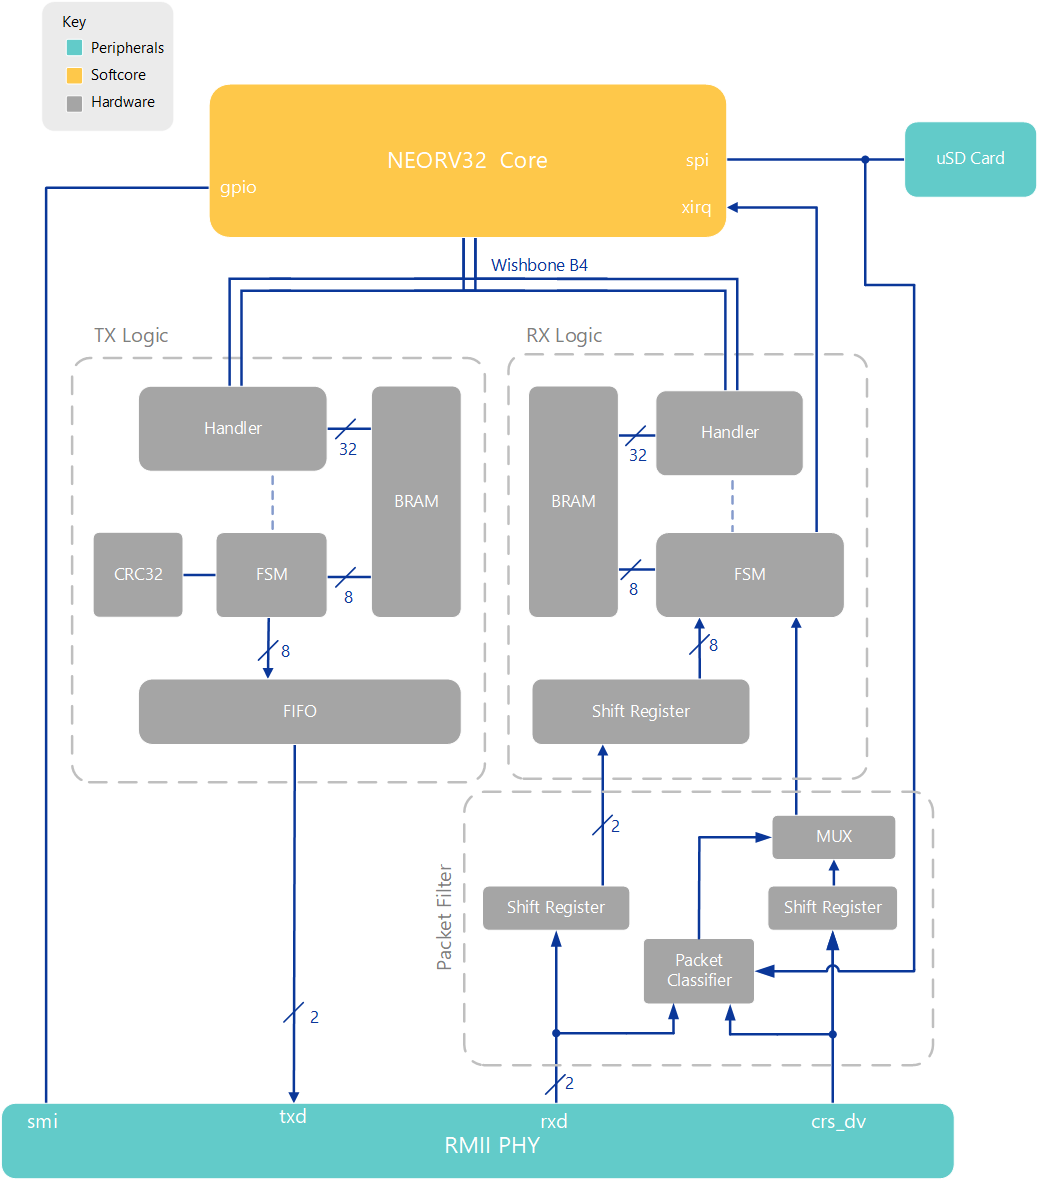
\includegraphics[width=0.85\textwidth]{Images/SoCArchitecture.png}
    \caption[System on Chip high level architecture]{System on Chip high level architecture.}
    \label{fig:soc_architecture}
\end{figure}

\newpage

\noindent Since the design is only concerned about incoming filtering, the packet filter was only placed between the RMII PHY and the MAC. By filtering at the RMII interface level, the Ethernet MAC is indifferent to the filter and ultimately doesn't care about it. This allows for a simpler modular design compared to integrating the filter in the MAC hardware. This filter consists of classifier (discussed in section \ref{sec:packet_classifier}) which would determine whether to forward or block an incoming packet.

To do the filtering itself, a shift register can be used to essentially delay the inputs from the RMII PHY until the packet classifier has determined whether to forward or drop the packet. A simple MUX can then be used to either allow the packet to enter the wishbone MAC or to not. 

As the hardware in the MAC only processes the input if crs\_dv is high, we only need to gate the crs\_dv and can always have the rxd lines always attached. However, these should also go through a shift register.

By doing this, it means that we can operate the filter at wirespeed with the only downside is the extra latency that the shift registers bring. The delay that these registers add to the latency can be found to be $T_{latency} = N\times T_{clk}$ where $N$ is the size of the registers. In the design a size of 224 ticks was used. This is because at a minimum, the packet classifier needed to input a maximum of $22 + 24 + 4 = 50$ bytes (22 for MAC headers including preamble, maximum 24 bytes for IP header and 4 bytes for the TCP/UDP headers (only need to check the source and destination port)) need to be processed. As there are four clock cycles per byte the needed register size is $50 \times 4=200$ for the data to propagate to the end of the registers after the packet classifier has determined whether to drop or allow the packet. Importantly this does not affect the speed/bandwidth of the connection. 


It is assumed that any traffic leaving from the device is safe and trusted. In a larger network where there are several devices behind the firewall, it may be desirable to also have a packet filter on the output. 


% amalgamates 








\subsection{Ethernet Media Access Controller}
\label{sec:ethernet_mac}
The advantage of using an FPGA is that custom hardware can be designed for specific tasks. In this design the MAC layer was done in hardware to free up the microprocessor by handling the lower level logic. 

This MAC was implemented as a memory-mapped peripheral which used the MCU's Wishbone B4 classic interface. This then made it easily accessible over the memory address space of the MCU.  



The hardware can be broken down into two main sections: the transmit logic and receive logic. 

In the receive logic, there are two main functions, one that stores the incoming frame into BRAM and then another to interface the BRAM with the Wishbone interface. On the input side the data is shifted into a 8bit wide shift register - shown in figure \ref{fig:soc_architecture}. While crs\_dv is asserted, after every four clock cycles (modulo four since 2 bits is received at a time) the contents of the shift register is stored into BRAM. After each byte has been added to BRAM, a counter is incremented to store the next byte in the next index. The end of the packet is signified when crs\_dv is deasserted, at which point the payload length is stored for use when the processor receives the frame over the wishbone interface. After the first two bits equals "01" (first 2 bits of the preamble) have been received, a trigger output is asserted so that it can fire a CPU interrupt.

On the wishbone side of the receive logic, only read requests are accepted and processed. A register access returns the payload size of the received frame to help the driver (section \ref{sec:ethernet_mac_driver}) identify how much data it needs to extract from the hardware buffer. When accessing the BRAM memory locations over the Wishbone interface two things are considered. The first is that an offset of eight is needed since the BRAM stores the preamble and SFD which is not wanted by the processor. The second is that the payload is stored in 8bit values whereas the wishbone interface can send 32bits at once. Therefore some conversion between the memory addresses and the memory accesses to BRAM take place. 


\newpage

\begin{lstlisting}[language=VHDL, caption=Wishbone access logic for Ethernet receive]
if wb_i_stb = '1' and wb_i_addr(31 downto 16) = x"1338" then 
    wb_o_ack <= '1';
    if wb_i_we = '0' then -- Ensure write enable is reset to read.
        if wb_i_addr(15 downto 0) = MAC_DAT_SIZE then -- Payload size
            wb_o_dat <= std_logic_vector(to_unsigned(payloadLen, 32));
        elsif wb_i_addr(15 downto 0) >= x"0008" and wb_i_addr(15 downto 0) <= x"05F8" then -- BRAM access
            virtAddr := to_integer((unsigned(wb_i_addr(15 downto 0)) - 8));
            wb_o_dat <= FRAME_BUFFER(virtAddr) &  FRAME_BUFFER(1 + virtAddr) & FRAME_BUFFER(2 + virtAddr) & FRAME_BUFFER(3 + virtAddr);
        end if;
    end if;
else
    wb_o_ack <= '0';
end if;
\end{lstlisting}

\noindent By splitting the address over 2 if conditions, the amount of resources can be greatly reduced as the nested if conditions only need to compare 16bits instead of 32bits each time. Another important design decision is that this version of the Ethernet MAC does not validate the FCS after receiving a packet, instead it assumes it's a valid packet. 


The transmit logic is broken down into three parts: Wishbone handler, main FSM and RMII conversion. The process of creating and sending an Ethernet frame starts with the processor sending data over the Wishbone interface. Like the receive logic, there are two types of commands that can be sent over the Wishbone interface, one that controls the logic, the other that stores payload data into BRAM. There are three configuration commands, one to initialise the hardware and FSM, another to start the transmission of data (used after all data has been transferred into BRAM) and one to set the payload length of the packet. The other register addresses allow the processor to store the payload in the frame buffer (BRAM). See figure \ref{fig:bram_frame_format} for the format of data in BRAM. The preamble, SFD and FCS are left out as these are appended in hardware. To be accurate, this is a quasi-MAC as the MAC addresses and type fields in the header (expanded view of payload in figure \ref{fig:bram_frame_format}) are populated in software. 

\begin{figure}[h!]
    \centering
    \begin{tikzpicture}

        % First bytefield
        \node (a) {
            \begin{bytefield}{8}
                \bitbox{8}{Preamble} & \bitbox{4}{SFD} & \bitbox{16}{Payload} & \bitbox{6}{Padding} & \bitbox{4}{FCS} 
            \end{bytefield}
        };

        % Expanded Payload
        \node[below=1cm of a.south] (b) {
            \begin{bytefield}{16}
                \bitbox{5}{D.Addr} & \bitbox{5}{S.Addr} & \bitbox{4}{Type} & \bitbox{14}[bgcolor=lightergray]{IP payload}
            \end{bytefield}
        };

        \node[right=0.5cm of b.east, anchor=west] {Populated in software};

        % Connection lines
        % Arrow from the left side of Payload to Field 1
        \draw[->] ([xshift=4.8cm]a.south west) -- ([xshift=0.35cm]b.north west);

        % Arrow from the right side of Payload to Field 3
        \draw[->] ([xshift=10.8cm]a.south west) -- ([xshift=10.75cm]b.north west);

    \end{tikzpicture}
    \caption{Format of frame in BRAM}
    \label{fig:bram_frame_format}
\end{figure}


\noindent Once a payload has been stored in the frame buffer, the main FSM takes control and at this point the CPU is free to do anything else. Since the FCS is calculated in hardware, the FSM resets the FCS hardware and begins to send the bytes to both the FCS hardware (to calculate the CRC32) and to a FIFO buffer. Once the payload has been transmitted to the FIFO, the resulting CRC32 FCS is sent out to the FIFO without missing a clock cycle. 

A FIFO buffer is used to cross the domains since the RMII interface is 50MHz at 2bits wide, whereas the bytes are stored as 8bit vectors in the frame buffer. This also allows the FSM to have a higher clock speed as well. The current implementation of the FSM uses a 80MHz clock signal, consequently the equivalent bit rate is 6/4 times larger than the output needed to the RMII interface. The FIFO used in this design, figure \ref{fig:fifo_diagram}, is slightly modified so that the read clock is one quarter the 50MHz output frequency since the FIFO itself returns 8 bits at a time. An FSM operating at 50MHz then sends each 2bit nibble out to the RMII PHY at a time in a circular fashion. The tx\_en line is asserted while the FIFO is non-empty.


\begin{figure}[h!]
    \centering
    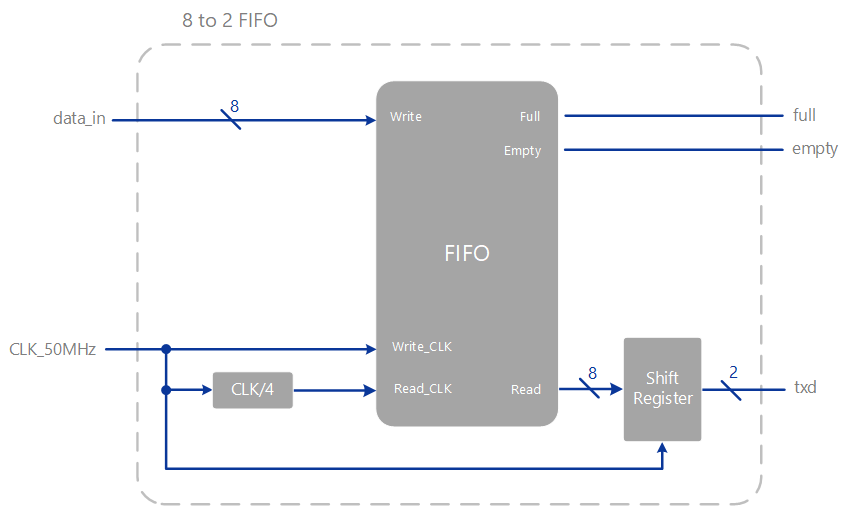
\includegraphics[width=0.75\textwidth]{Images/EthFIFO.png}
    \caption[8bit to 2bit FIFO used for RMII output]{8bit to 2bit FIFO used for RMII output.}
    \label{fig:fifo_diagram}
\end{figure}




\noindent The documentation for the NEORV32 states that all memory accesses that do not target specific processor-internal address regions (see appendix \ref{app:mem_address}) get forwarded to the external interfaces, such as the Wishbone interface. As such, there is a large block of unused memory between the IMEM and DMEM regions. The memory mapping, figure \ref{fig:memory_layout}, used in this design ranges from 0x13370000 to 0x133805F8.


% \begin{tikzpicture}[remember picture,overlay]
%     % Define coordinates for shading
%     \coordinate (top-left) at (3.95, -0.05);  % Adjust as necessary
%     \coordinate (bottom-right) at (10, -2.5); % Adjust as necessary
    
%     % Draw shading
%     \fill[gray!30] (top-left) rectangle (bottom-right); % Change gray!30 to your desired shading color and intensity
% \end{tikzpicture}

\begin{figure}[h!]
    \begin{center}
    
\begin{bytefield}{24}
% \memsection{ffff ffff}{0040 0000}{5}{Processor memory}\\
\memsection{1338 05F8}{1338 0008}{5}{RX PAYLOAD}\\
\memsection{1338 0007}{1338 0004}{2}{RX SIZE}\\
\memsectioncolour{1338 0003}{1337 6411}{3}{Unused}\\
\memsection{1337 6410}{1337 1004}{4}{TX PAYLOAD}\\
\memsection{1337 1003}{1337 1000}{2}{TX SIZE}\\
\memsection{1337 0003}{1337 0000}{2}{TX CONFIG}\\
% \memsection{1336 ffff}{0000 0000}{5}{Processor memory}
\end{bytefield}
\caption{Memory Address Layout}
\label{fig:memory_layout}
\end{center}
\end{figure}

This mapping is required for developing the driver (section \ref{sec:ethernet_mac_driver}) to access the correct registers.









\subsection{Packet Classifier}
\label{sec:packet_classifier}
Inspired by \cite{FastRecongifFPGAFirewall}, to further save MCU resources, the packet classification was done in hardware. Not only did this reduce the load on the MCU itself - giving it more time to do other things - it allowed the interface to run at \textit{'wirespeed'}. That is, at the full speed of the interface - 100Mbit/s. 

This was possible by having the rulset been evaluated in parallel as the data is coming into the firewall. This method however is not suitable for large rulesets as the fan-in and fan-out limit the maximum number of parallel comparisons. For every new rule, the number of gates grows exponentially. Hence a design decision of a maximum ruleset of size 8 was chosen. 

The way this classifier was designed was to be a \textit{'default-block'} where all connections were blocked except for the ones specifically whitelisted in the ruleset. The specific rules had a few options, namely the source IP address, destination IP address, source port, destination port and protocol could be configured. In addition to these, each field had a wildcard operator which allowed all values for that specific option to be classified. 


The design of the packet classifier hardware, inspired from \cite{FastRecongifFPGAFirewall} and shown in figure \ref{fig:packet_classifier_architecture}, stores the firewall rules in block memory. The rules are stored in BRAM as an array of 112 bits with the format shown in figure \ref{fig:pc_rule_format}.


\begin{figure}[h!]
    \centering

    \begin{bytefield}{8}
        \bitbox{6}{$Wildcard$} & \bitbox{5}{$IP_{Dest}$} & \bitbox{5}{$IP_{Src}$} & \bitbox{6}{$Port_{Dest}$} & \bitbox{6}{$Port_{Src}$} & \bitbox{6}{$Protocol$} 
    \end{bytefield}
    
    \caption{Format of rules stored in BRAM}
    \label{fig:pc_rule_format}
\end{figure}


\noindent The wildcard attribute signifies whether to allow all possible combinations (in other words, disregard) for the positional attribute where the most significant bit refers to the $IP_{Dest}$ and the least significant bit refers to the $Protocol$.

An FSM then records the position of the incoming and configures the multiplexers on the BRAM to output the current property to the comparators where they compare with the shift register which contains the current field being classified. On a successful match, a bit is left set in the result register, otherwise clear if no match. Importantly, the bits only get set on the first iteration of the classification. 

After passing through all the fields, if there is any bit set in the results register, it indicates that a rule matched and that a packet should be forwarded. 


\begin{figure}[h!]
    \centering
    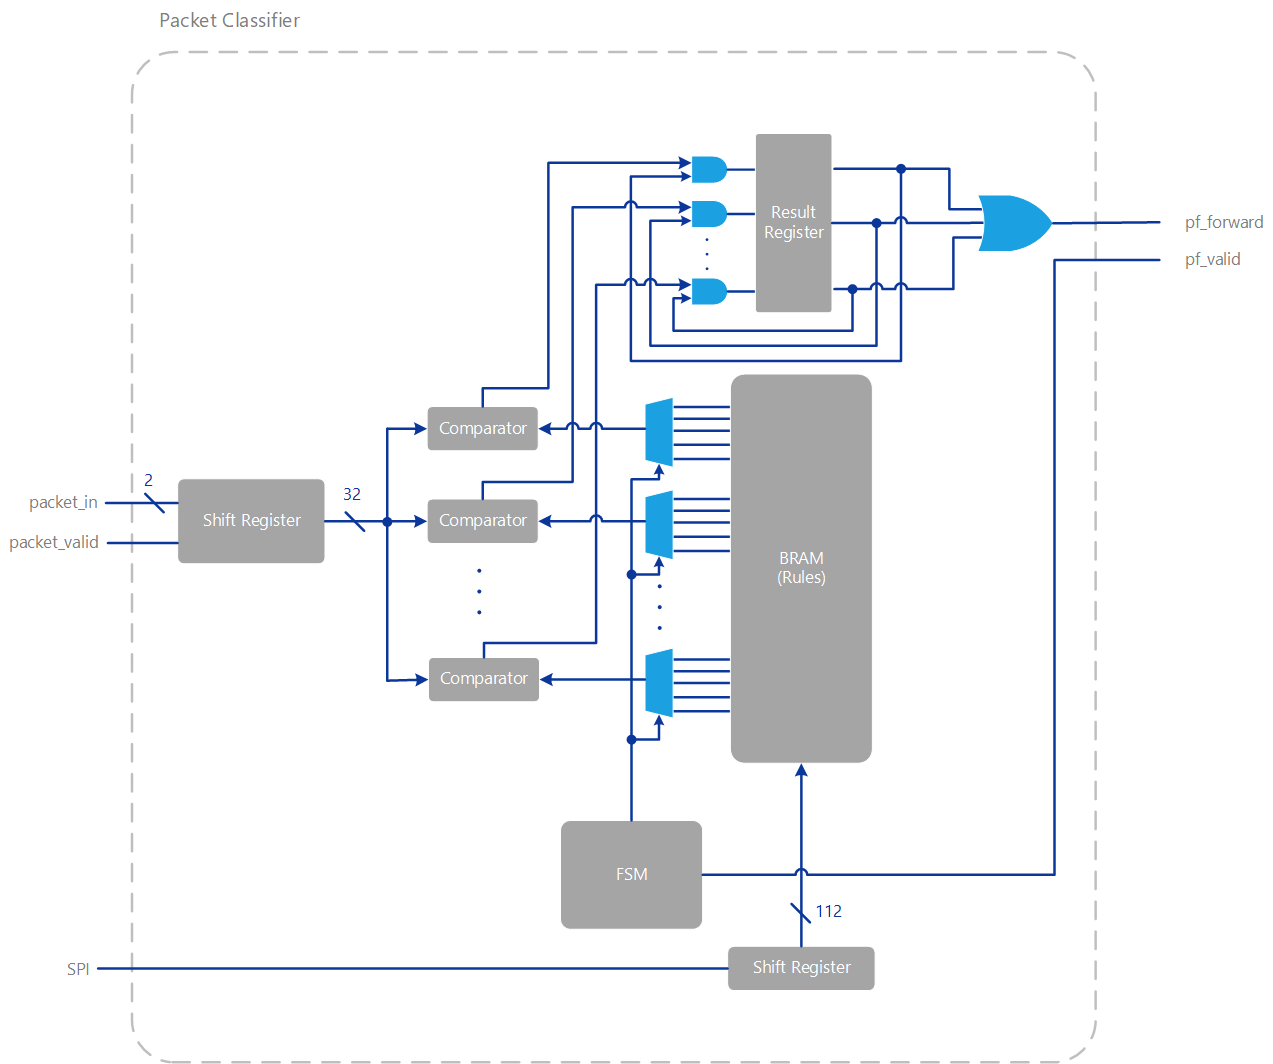
\includegraphics[width=1\textwidth]{Images/PacketFilterArchitecture.png}
    \caption[Packet classifier architecture]{Packet classifier architecture. Clock signals have been omitted.}
    \label{fig:packet_classifier_architecture}
\end{figure}

\noindent This reduces the required resources as only 1 set of comparators are needed, which is important as for each rule that exists, another comparator is needed. In this design, there are a total of 8 comparators, 8 multiplexers and the results register is 8bits wide. 

A more resource efficient design is possible at the cost of latency. This is one of the critiques of the design mentioned in \cite{FastRecongifFPGAFirewall} as multiple clock cycles would be needed to classify the headers. In theory the clock speed could be faster than Ethernet frequency and as only two bits from the RMII interface are processed at a time, it could be a viable alternative, however this may likely fall apart when higher speeds are required. 


Several options exist for configuring the ruleset in the packet classifier such as: Wishbone, I2C, UART, SPI or a completely custom solution. For simplicity, SPI was used in configuring the packet filter. Importantly, data would only flow in one direction, from the microcontroller to the classifier and not the other way round. This means that the microcontroller needs to keep the state of the rules inside the packet filter and needs to resend the rules to be sure of the configuration. This is not an issue as the rules need to be stored in flash on the microSD card to keep settings between power cycles. The format, figure \ref{fig:spi_message_format} that the SPI hardware expects is similar to how it's stored in BRAM to make it quick and easy to transfer.

\begin{figure}[h!]
    \centering

    \begin{bytefield}{8}
        \bitbox{6}{$Index$} & \bitbox{6}{$Wildcard$} & \bitbox{5}{$IP_{Dest}$} & \bitbox{5}{$IP_{Src}$} & \bitbox{6}{$Port_{Dest}$} & \bitbox{6}{$Port_{Src}$} & \bitbox{6}{$Protocol$} 
    \end{bytefield}
    
    \caption{Format of SPI messages}
    \label{fig:spi_message_format}
\end{figure}



\noindent Notably, the data is received into a shift register and after all bits have been received the BRAM is updated at the corresponding index in a single clock cycle.








\section{Firmware}
\subsection{Ethernet drivers}
\label{sec:ethernet_mac_driver}

Since the Ethernet hardware was custom, drivers were needed to interface with the hardware in software. There were two types of commands that were needed, first the RMII serial management interface (SMI) and secondly the MAC drivers - the drivers that would handle the data.  The SMI interface is used to control the mode of operation of the PHY chip including the speed, Auto-MDIX, duplex settings. The LAN8720A datasheet, (\cite{LAN8720ADatasheet}) provided some details (seen in figure \ref{fig:smi_packet_structure}) into how the protocol operated. The datasheet also outlined that a maximum frequency of 2.5MHz, but no lower bound. As such the interface was \textit{'bitbanged'} with GPIO pins to reduce complexity. The maximum switching frequency of the NEORV32's GPIO was measured to be $\approx 1$MHz, thus no additional delays were needed in the code and that the GPIO pin could be toggled at the fasted speed possible. 


\begin{figure}[h!]
    \centering
    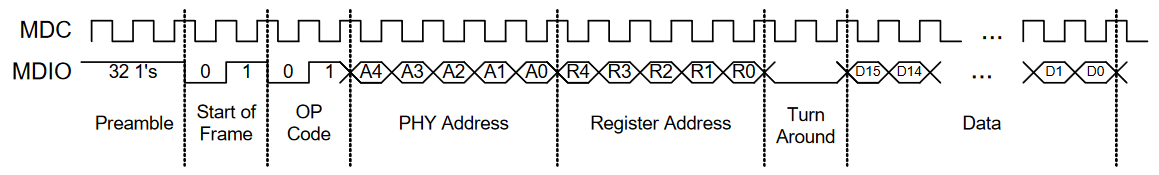
\includegraphics[width=0.75\textwidth]{Images/SMIWriteStructure.png}
    \caption[SMI Write message structure]{SMI Write message structure. \cite{LAN8720ADatasheet}}
    \label{fig:smi_packet_structure}
\end{figure}

\noindent On power up the RMII interface would be set to full duplex, 100Mbps and auto-negotiate in accordance to the LAN8720A datasheet. 10Mbit and half duplex modes were excluded from the design as further hardware design would be required.  


As the Ethernet hardware used the Wishbone interface, the register locations were mapped into the processors address space. Accessing these registers is analogous to accessing any other variable in memory, using pointers to the memory address. As an example, to access memory location \codebg{0x12345678} the following C code can be used \codebg{*(volatile uint32_t *) 0x12345678}


To simplify the design and improve readability, a range of macros was setup, such example of macros can be seen below. 

\newpage

\begin{lstlisting}[language=C, caption=Python example]
#define ETH_MAC_TX_BASE 0x13371000
#define ETH_MAC_CMD_BASE 0x13370000

#define ETH_MAC_CMD  (*(volatile uint32_t *)ETH_MAC_CMD_BASE)
#define ETH_MAC_TX ((EthMacTx *) ETH_MAC_TX_BASE)

typedef struct __attribute__((__packed__))  {
    volatile uint32_t SIZE;
    volatile uint32_t DATA[375]; // 1500 / 4 = 375.
} EthMacTx;
\end{lstlisting}

\noindent This allowed for the connected wishbone Ethernet to be accessed like any other register in the embedded system. 


There are three fundamental functions that the driver itself must fulfill, initialisation, send data and receive data. The initialisation resets the Ethernet MAC and resets the interrupt registers. 

The send method is also trivial, but importantly it takes in two parameters, the first is an array of data to send and the second is the amount or length of the data. Like with the SMI interface, these instructions and data transfers were actioned without any delays as the hardware was capable of handling the native speed of the processor. After the data had been transferred, the hardware is instructed to send out the packet. There is no need to provide the FCS as this is calculated on the fly in hardware. 

Similarly, a receive method was created that took in a buffer to store the bytes into as it transfers the data into memory from the registers. Both the transmit and receive functions handled the data translation from 32bit values over the wishbone interface to 8bit bytes in software. In addition to this, as the Ethernet hardware used external interrupts to signal to the processor that there is an Ethernet packet ready for processing. This would use direct task notifications to signal to other functions in the code to call the receive method. 


\subsection{SD card drivers}
\label{sec:microsd_drivers}
To use a micro SD card, drivers must be created so that the card can be initialised, written to and read from. More precisely, in accordance to the  documentation for the FreeRTOS-Plus-FAT file system, the driver had to implement a function that reads sectors from the media and one that rights sectors to the media. 

Unlike the Ethernet MAC, initialising a MicroSD card isn't as trivial and requires multiple steps. A guide online for AVRs\footnote[1]{See: http://www.rjhcoding.com/avrc-sd-interface-1.php} was followed and the code was ported to the NEORV32 system. In essence, the SPI interface was initialised with a clock divisor of 1 and a prescalar of 3, several commands were sent and received from the SD card and then it was put into IDLE mode after increasing the speed of the SPI interface to have no clock divisor and a prescalar of 1.

Similarly, the same guide was followed to implement the read and write sector functions. Importantly, these functions would read and write a whole block at a time. On a microSD card, a block is considered to be 512 bytes. 


In addition to these, a simple function to determine if a SD card is present in the slot was also implemented to warn the user if data was attempted to be written to or read from without a physical card in the slot. 





\subsection{Packet classifier drivers}
\label{sec:packet_filter_driver}
An initialisation function was created to enable and configure the SPI interface on the microprocessor for mode 0, and with no clock diviser and a prescalar of 1. The SPI hardware for the classifier can handle speeds in excess of 80Mhz (seen in section \ref{sec:timing_constraints}), hence there was no need to slow down the clock. Moreover, calling this initialise function is only required if the microSD card intialise function has not been called. 

A single function was created that takes in all the attributes needed in the packet filter and that sends these out in the correct order and format to the hardware. 








\section{Software}

\subsection{Real Time Operating System}
In addition to simplifying the software, an RTOS was used to allow the use of network TCP stacks and handle multiple concurrent connections at a time. FreeRTOS version V10.4.4 was used due to its familiarity and compatibility with the NEORV32 MCU. FreeRTOS also had integration with their own filesystem (section \ref{sec:freertos_filesystem}) and TCP/IP stack (section \ref{sec:freertos_tcpip_stack}).

\subsection{Filesystem}
\label{sec:freertos_filesystem}
The FreeRTOS-Plus-FAT filesystem library was used to allow the system to read and write files (such as web assets) to a microSD card. The library is managed by FreeRTOS and is DOS compatible which allows FAT32 formatted drives to work. Other popular filesystem modules such as FatFS\footnote[1]{http://elm-chan.org/fsw/ff/00index\_e.html} and LittleFS \footnote[2]{https://github.com/littlefs-project/littlefs} were also considered, but did not have the same level of integration and active support as the FreeRTOS option. 

The library then uses the microSD card drivers (section \ref{sec:microsd_drivers}) to access the disk. 


\subsection{Network Stack}
\label{sec:freertos_tcpip_stack}

Two main options for the network stack were available, LwIP and FreeRTOS-Plus-TCP. The main concern with LwIP was that it was not threadsafe and had memory issues. In addition to this, as FreeRTOS was chosen as the RTOS, their own TCP stack had tighter integration. The stack provides a Berkeley sockets API which is the same used in full-blown operating systems such as Linux. It also includes support for ARP, DHCP, DNS and ICMP protocols, which were used throughout this project. 

Like with the filesystem library, the stack needed to be ported to the NEORV32 processor and importantly the custom Etherent hardware. In addition to the transmit, receive and initialisation methods, functions to return random numbers were needed. These are for the TCP sequence numbers and are required to truely random for security. As such, the hardware based true random number generator in the NEORV32 core was used. 

The network stack was configured to use DHCP to automatically acquire an IP address from a DHCP server on a network so that when it's transported between networks it can dynamically get a new IP address and can be accessed without needing to reconfigure the device. The device can then be given a static IP through the DHCP server by creating a static mapping. This will then prevent the DHCP server from assigning the desired IP address to another device accidentally. 

\subsection{Web application}
With the resource constraints of the RISC-V microcontroller in mind and other design requirements, Vue.js was chosen as the framework of choice for developing the web application. Vue.js is a framework for developing componentised single page applications. Although technically single page, the Javascript it compiles handles routing between web pages on the client side in Javascript. This means that once the initial page has loaded, no additional server requests need to be made to change page. To make the website appear dynamic, an API can be used to fetch data and statistics from the device itself. These HTTP API requests are much smaller than the requests needed to load the webpage initially. This results in very low network traffic between the client and server, perfect for embedded systems. 

For styling, TailwindCSS was used to help style the webpages to give the webapp a contemporary feel. 

The webapp consisted of 3 main pages, the index or home page, about page and config page. The home page, figure \ref{fig:webapp_home} showed statistics such as total and blocked packet count, and statuses for a few tasks on the microcontroller. These tasks, through an API call, can be toggled on and off to save resources. An uptime reading is also present. These values are updatable by clicking the 'refresh' button.

\begin{figure}[h!]
    \centering
    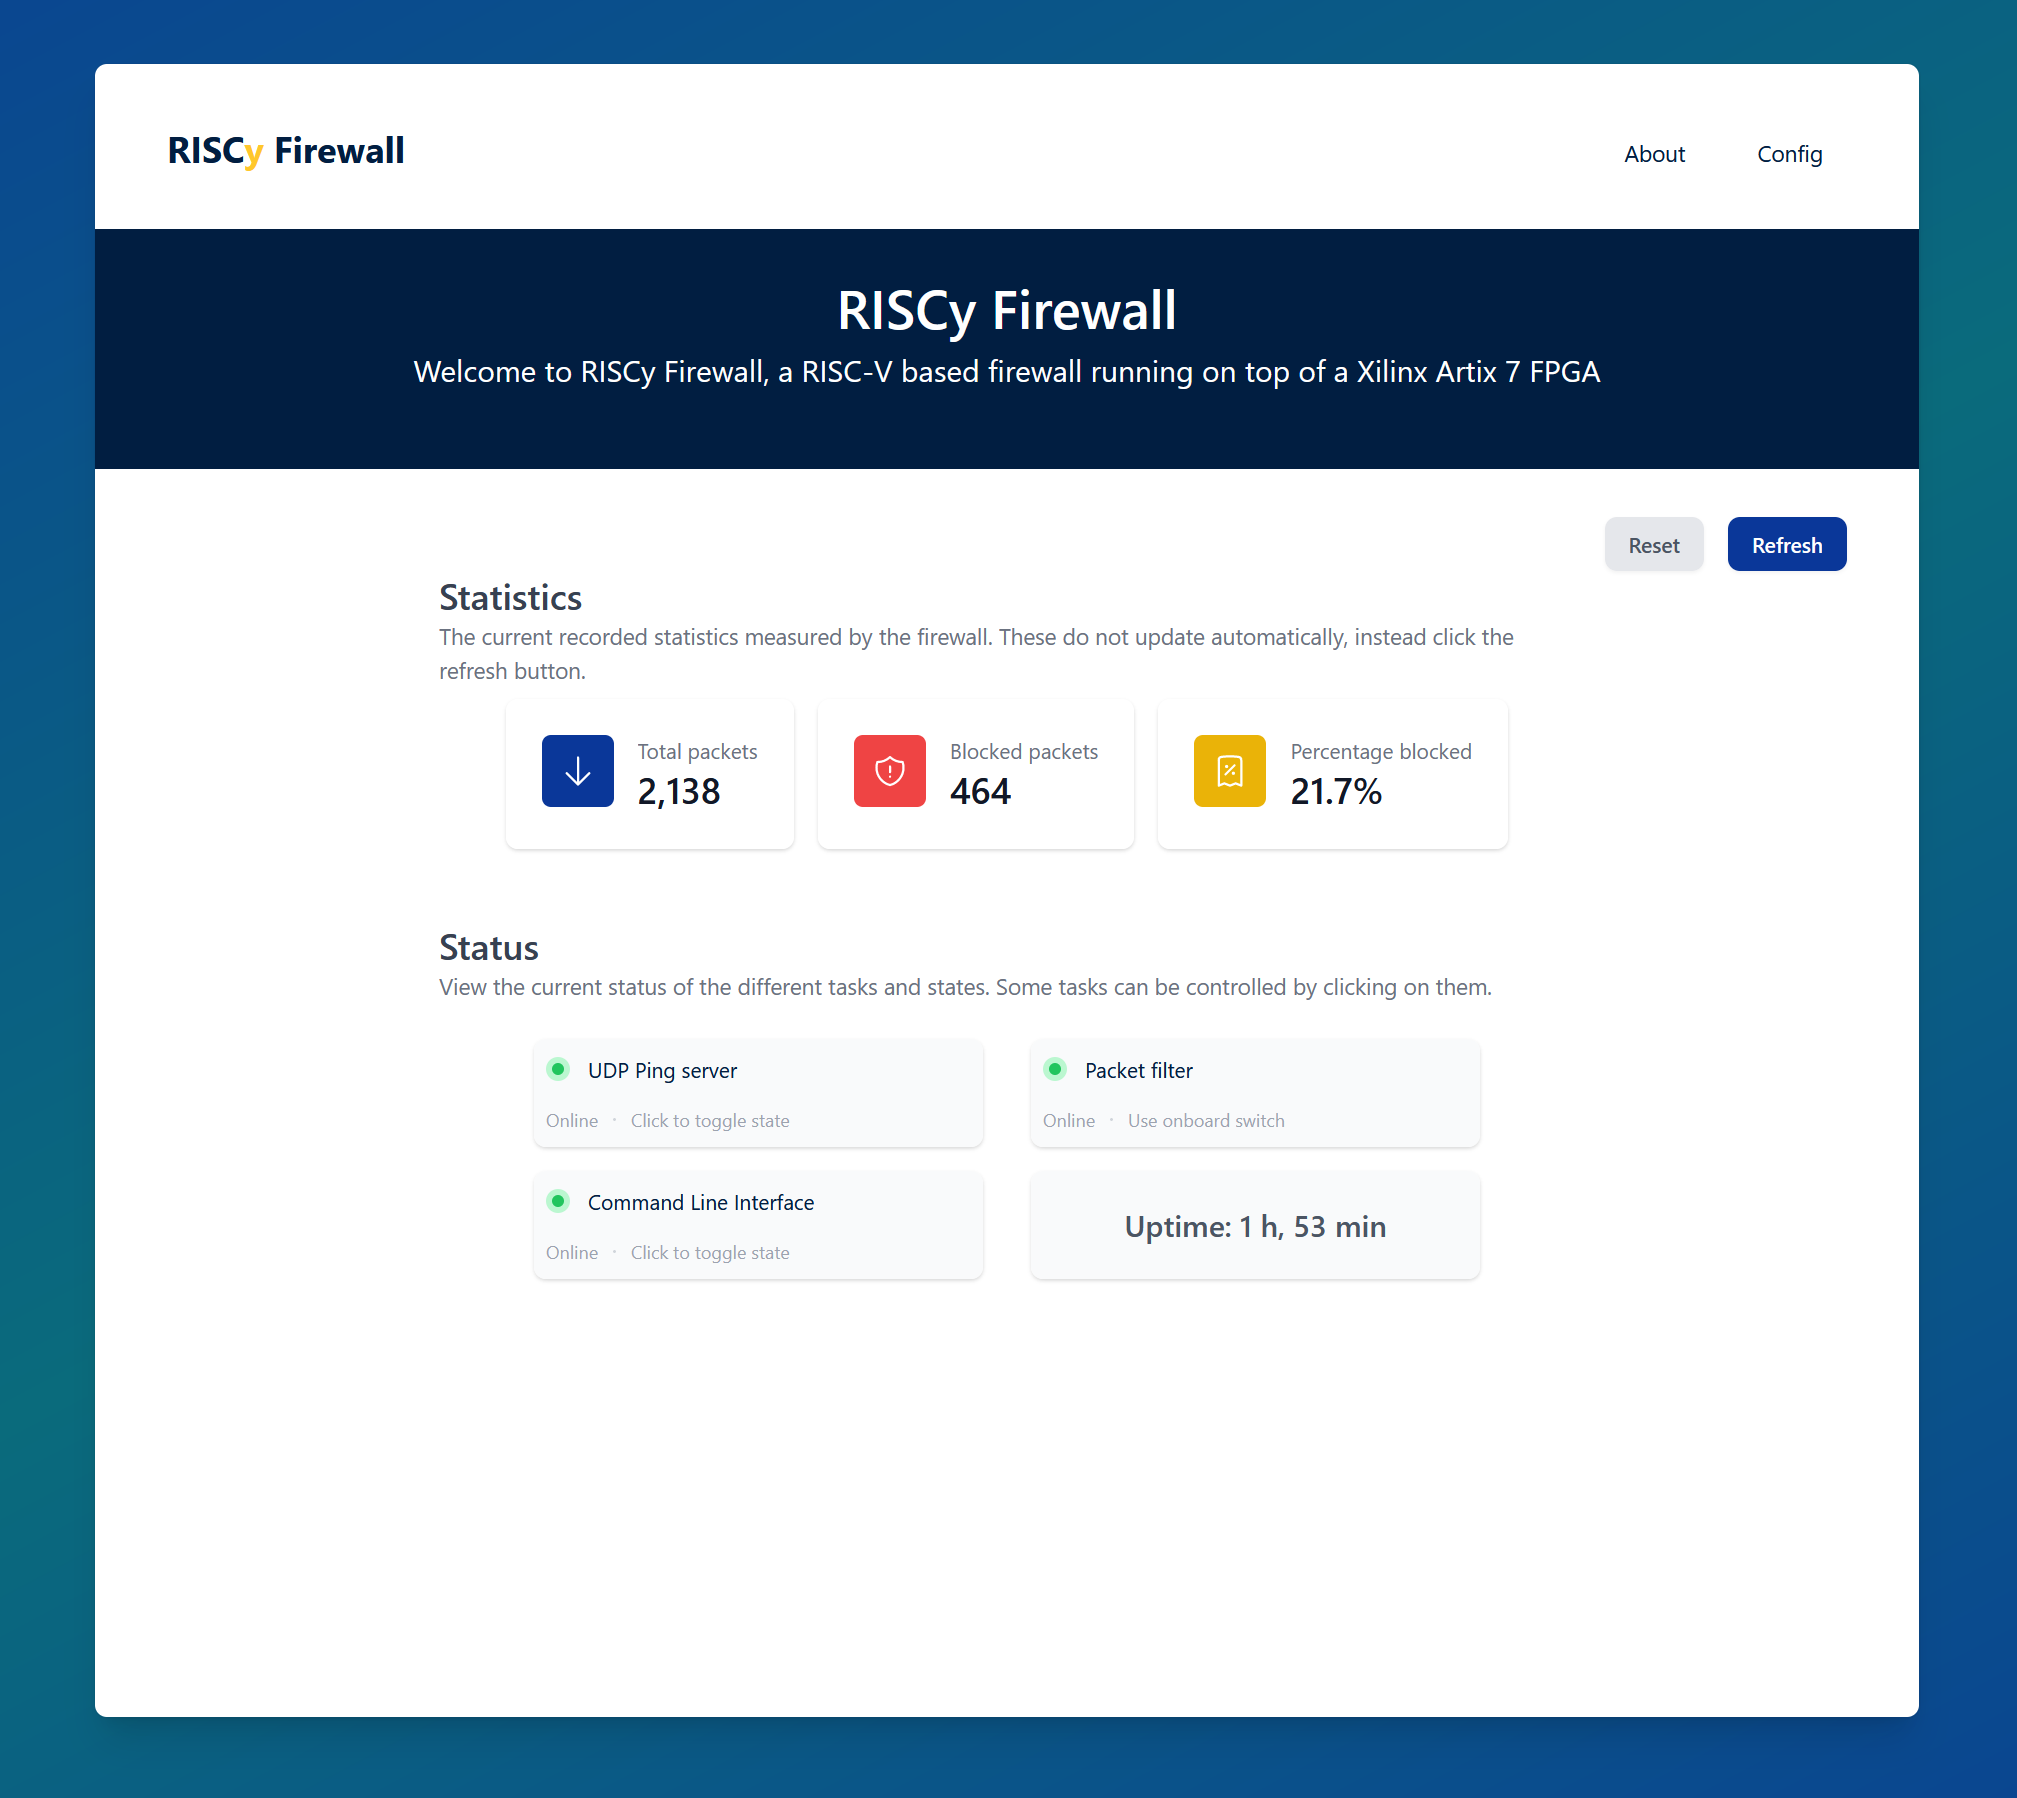
\includegraphics[width=0.75\textwidth]{Images/homepage_small.png}
    \caption[Screenshot of homepage on webapp]{Screenshot of homepage on webapp.}
    \label{fig:webapp_home}
\end{figure}

The configuration page, (figure \ref{fig:web_app_config} shown in appendix \ref{app:additional_webpages}) is where the user configures the firewall rules. The rules first need to be loaded which is requested through an API request. This API request reads the rules from the microsd card, sets the rules (for consistency) and then returns them in the response packet. When the user saves a set of rules, an API request is made which first applies the rules and then saves the rules to the microsd card so that the changes are persistent. 

An about page (figure \ref{fig:web_app_about} shown in appendix \ref{app:additional_webpages}) was also created for demonstration purposes and contained an image.

In addition, as this is all client side and compiles to HTML, CSS and Javascript, no special webserver is required for things such as server side rendering.


\subsection{Webserver}
A simple HTTP webserver running on top of a TCP server was used to serve the webpages for the project. FreeRTOS give an example of how to setup a TCP and HTTP server that uses the FAT filesystem to get the content such as the HTML, CSS and Javascript files. All the TCP webserver has to do is determine the route requested by the client, based on this it knows whether to read a file from the micro SD card and send it over multiple TCP packets or if it needs to respond with raw data like in the case of the API. Regardless of the type of request, a response is formed in the standard HTTP 1.1 format given in RFC2616 \cite{rfc2616}.


\subsubsection{API server}
A subset of the webserver is the API server itself. To make the design simpler, an API was created so that the interface to set and get the firewall rules was independent of the web content. The way the software distinguishes between requests to load a webpage and the API server itself is by inspecting both the route/URL (pcUrlData) and the method type (GET, POST, PUT).

For setting the firewall rules, a POST request to the \textit{'/api/firewall'} endpoint can be made. The body of the request would contain the rule in the following format

\[
payload=Index | Wildcard | IP_{Dest} |  IP_{Src}  | Port_{Dest} |  Port_{Src} | Protocol
\]

Where $|$ is the concatenation operator and all fields are in hexadecimal. As an example, to insert a rule at index 0, and with a wildcard operator for all items with a destination IP of 10.20.1.120, source IP of 10.0.0.159, source and destination port of 80 and a protocol of TCP, the following body would need to be sent to the API: \codebg{payload=003F0A1401780A00009F0050005006}. The API server then takes the necessary action and applies the rule to the packet filter by calling the methods in the packet filter driver (section \ref{sec:packet_filter_driver}).



\subsection{Command line interface}

To aid with debugging the FreeRTOS-Plus-CLI framework was used. This would easily allow certain actions to be executed on demand without the need to reflash or reset the device each time. Such examples include configuring the PHY, Ethernet MAC, sending ICMP packets and filesystem related commands. In addition, the firewall rules can be set from the CLI in the event that the firewall blocks HTTP connections. 
